\documentclass{article}

\usepackage{graphicx}
\usepackage{tikz}
\usepackage{tikzsymbols}
\usetikzlibrary{calc,patterns,shapes.geometric}
\pagestyle{empty}
\usepackage[margin=0pt]{geometry}
\geometry{papersize={14in,12in}}

\def\centerarc[#1](#2)(#3:#4:#5){\draw[#1] ($(#2)+({#5*cos(#3)},{#5*sin(#3)})$) arc (#3:#4:#5);}

\begin{document}
	\begin{figure}
		\centering
		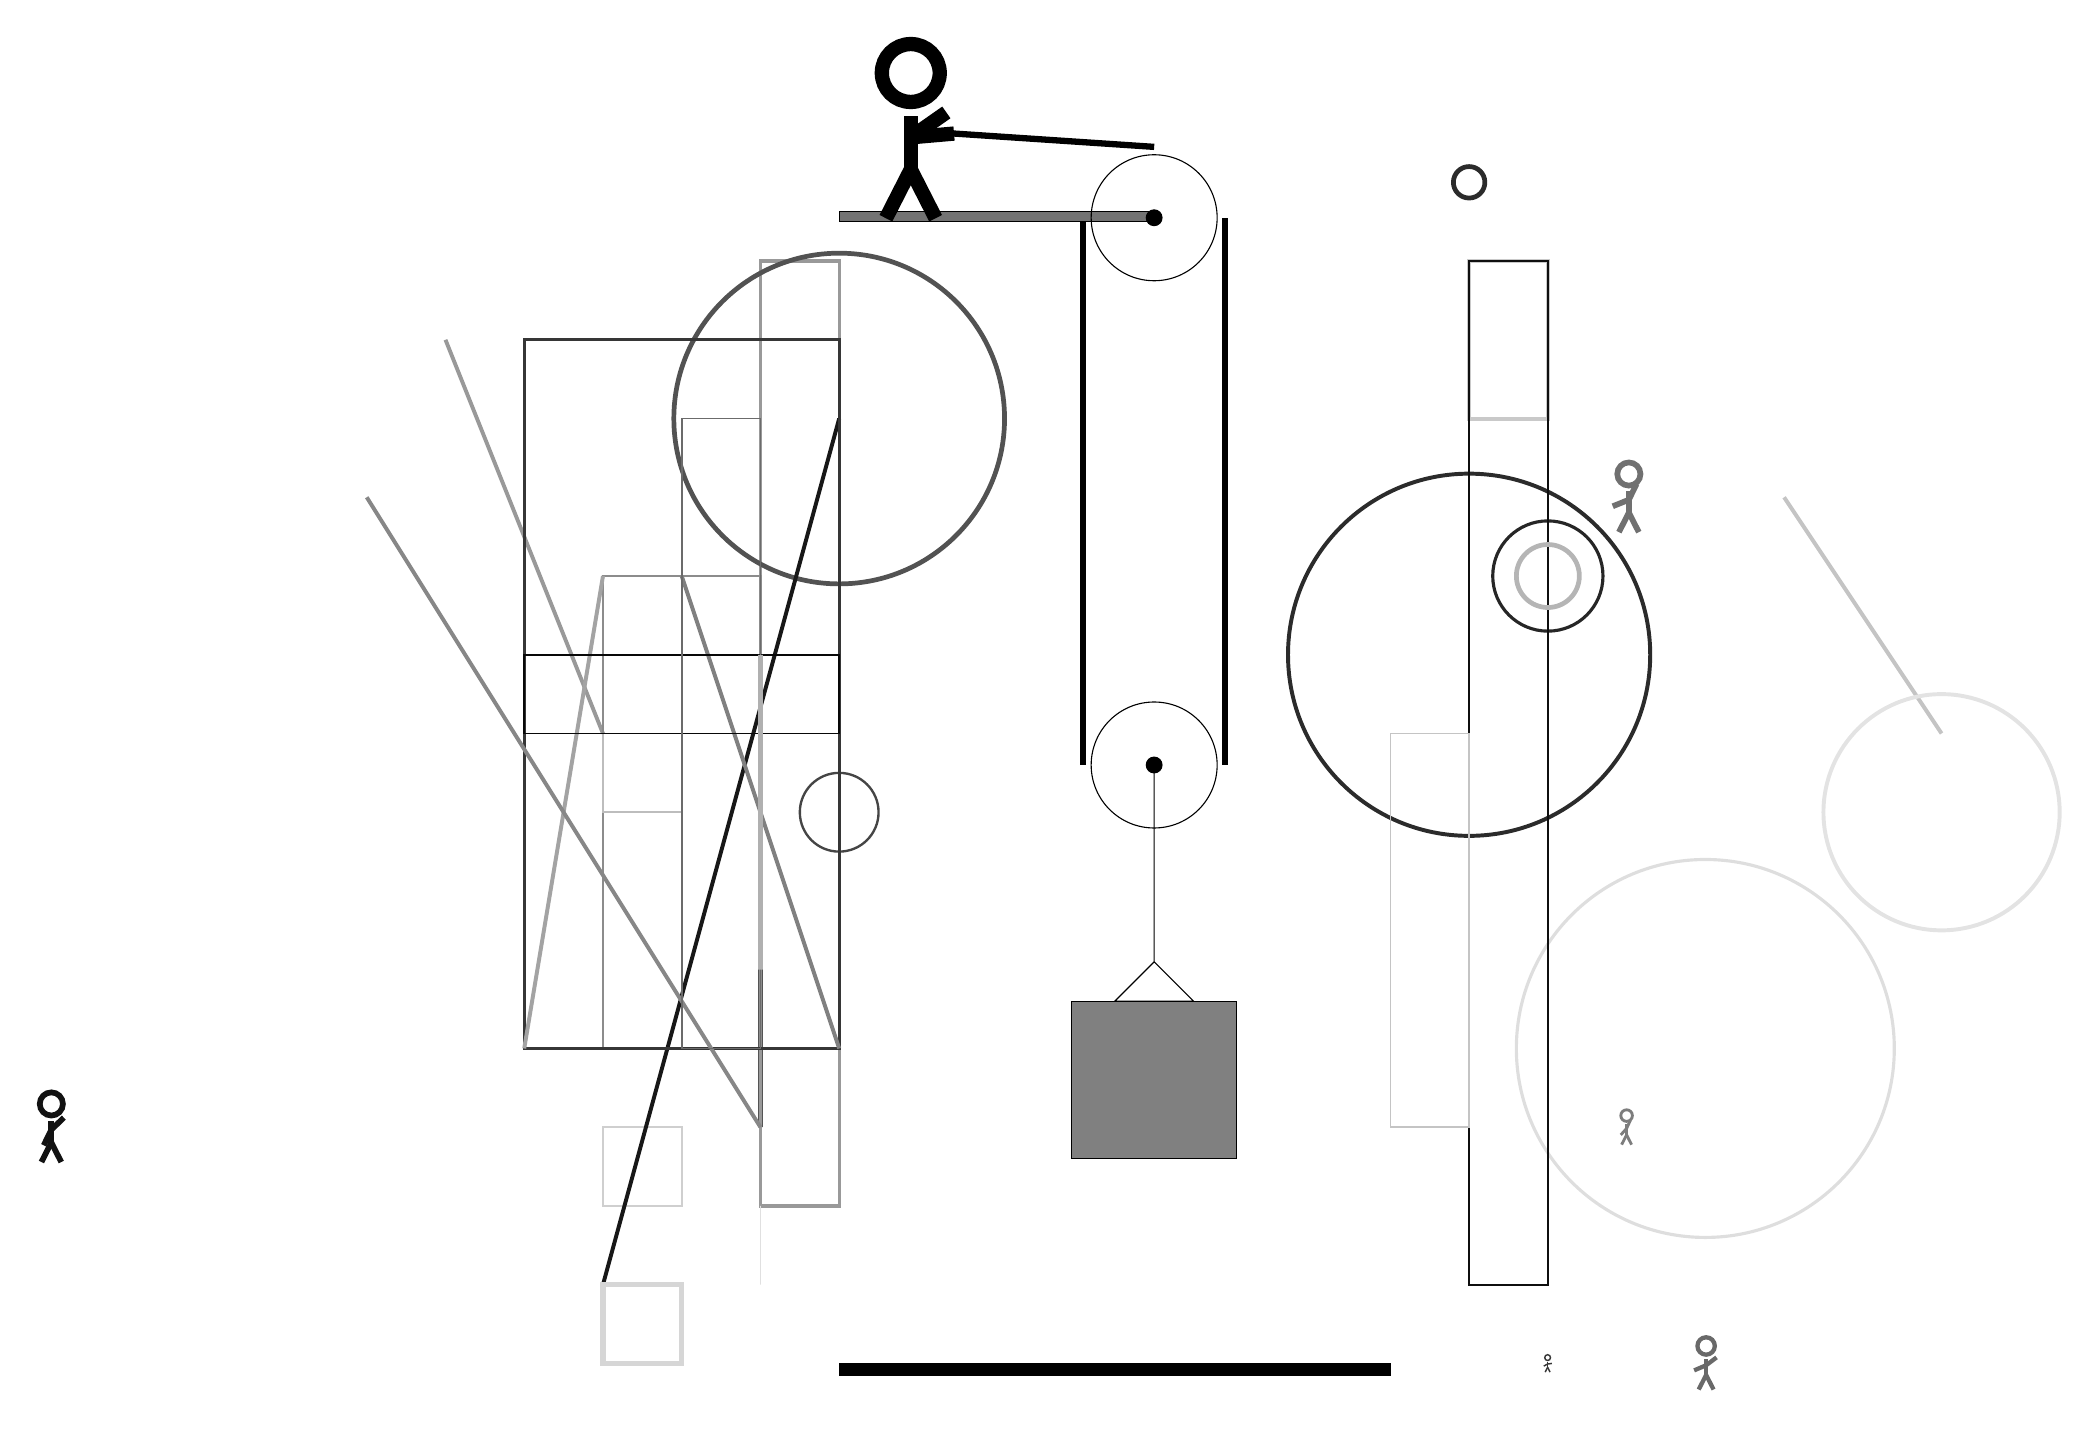
\begin{tikzpicture}
			%%%%% START %%%%%
			
			\draw[fill=black!55] (-2, 11.5) rectangle (2, 11.625);
			
			\draw (2, 4.6) circle (0.8);
			\draw[fill=black] (2, 4.6) circle (0.1);
			
			\draw (2, 11.55) circle (0.8);
			\draw[fill=black] (2, 11.55) circle (0.1);
			
			\draw (2, 4.6) -- (2, 2.1) -- (1.5, 1.6) -- (2.5, 1.6) -- (2, 2.1);
			\draw[fill=black!50] (0.95, 1.6) rectangle (3.05, -0.4);
			
			\draw[line width=0.8mm] (1.1, 11.5) -- (1.1, 4.6);
			\centerarc[line width=0.8mm](2, 4.6)(180:360:0.9);
			\draw[line width=0.8mm](2.9, 4.6) -- (2.9, 11.55);
			\centerarc[line width=0.8mm](2, 11.55)(0:90:0.9);
			\draw[line width=0.8mm](2, 12.45) -- (-1, 12.65);
			
			\draw [line width=0.3mm, color=black!73](-2, 4) circle (0.5);
			
			\draw [line width=0.5mm, color=black!83](6, 6) circle (2.3);
			\draw[line width=0.7mm, color=black!67] (-3, 5) rectangle (-3, 0);
			\draw[line width=0.4mm, color=black!40] (-2, -1) rectangle (-3, 11);
			\draw[line width=0.5mm, color=black!40](-7, 10) -- (-5, 5);
			\draw[line width=0.2mm, color=black!19] (-4, -1) rectangle (-5, 0);
			\node[line width=0.5mm, color=black!93] at (-12, 0) {\Strichmaxerl[4][64][44]};
			\draw [line width=0.4mm, color=black!13](9, 1) circle (2.4);
			\node[line width=0.2mm, color=black!56] at (8, 8) {\Strichmaxerl[4][22][64]};
			\node[line width=0.3mm, color=black!51] at (8, 0) {\Strichmaxerl[2][48][65]};
			\draw[line width=0.3mm, color=black!45] (-3, 7) rectangle (-5, 1);
			
			\draw [line width=0.6mm, color=black!83](6, 12) circle (0.2);
			\draw [line width=0.6mm, color=black!68](-2, 9) circle (2.1);
			
			\draw[line width=0.2mm, color=black!26] (-4, 4) rectangle (-5, 5);
			\draw[line width=0.5mm, color=black!91](-5, -2) -- (-2, 9);
			\draw[line width=0.7mm, color=black!16] (-4, -2) rectangle (-5, -3);
			
			\draw[line width=0.5mm, color=black!23](10, 8) -- (12, 5);
			
			\draw [line width=0.4mm, color=black!85](7, 7) circle (0.7);
			\draw[line width=0.2mm, color=black!12] (-3, -1) rectangle (-3, -2);
			
			\draw[line width=0.4mm, color=black!79] (-2, 1) rectangle (-6, 10);
			\draw[line width=0.5mm, color=black!21] (7, 11) rectangle (6, 9);
			
			\node[line width=0.6mm, color=black!79] at (7, -3) {\Strichmaxerl[1][28][8]};
			\draw[line width=0.3mm, color=black!94] (6, 11) rectangle (7, -2);
			\draw[line width=0.5mm, color=black!50](-2, 1) -- (-4, 7);
			\node[line width=0.6mm, color=black!59] at (9, -3) {\Strichmaxerl[3][23][37]};
			
			\draw[line width=0.2mm, color=black!23] (5, 0) rectangle (6, 5);
			\draw[line width=0.5mm, color=black!36](-6, 1) -- (-5, 7);
			\draw [line width=0.6mm, color=black!29](7, 7) circle (0.4);
			\draw[line width=0.5mm, color=black!47](-3, 0) -- (-8, 8);
			
			\draw[line width=0.2mm, color=black!97] (-2, 6) rectangle (-6, 5);
			\draw[line width=0.2mm, color=black!58] (-3, 1) rectangle (-4, 9);
			\draw[line width=0.6mm, color=black!31] (-3, 2) rectangle (-3, 6);
			\draw [line width=0.5mm, color=black!11](12, 4) circle (1.5);
			
			\node at (-1, 12.65) {\Strichmaxerl[10][-175][35]};
			
			\draw[fill=black] (-2, -3) rectangle (5, -3.15);
			
			%%%%% END %%%%%
		\end{tikzpicture}
	\end{figure}	
\end{document}